\documentclass[12pt, a4paper]{article}
\usepackage[margin = 1in, top=1.3in]{geometry}
\usepackage[english]{babel}
\usepackage[utf8]{inputenc}
\usepackage{fancyhdr}
\usepackage[fleqn]{amsmath}
\usepackage{mathtools}
\usepackage{tabto}
\usepackage{bm}
\usepackage{graphicx}
\graphicspath{{./images/}}
\usepackage[font=small,labelfont=bf]{caption}
 
\pagestyle{fancy}
\fancyhf{}
\rhead{\small{Shaan Ul Haque(180070053)\\ Samarth Singh (180050090) \\ Niraj Mahajan (180050069)}}
\lhead{CS-663 Assignment-4 : Question 5}
\rfoot{Page 5.\thepage}
 
\begin{document}
\vspace*{-22pt}
\section*{Question 5}
\subsection*{5.1: Reconstruction of Images Compressed by PCA}
\quad Using the PCA performed in the previous question, we compressed several images from the ORL dataset (d = 92x112 $\equiv$ 10304) to a mere k dimensional space for $k << d$. In this section, we reconstruct images back from their compressed state, and compare the information retention for different values of k
\vspace*{65pt}
\begin{figure}[h!]
    \centering
    \renewcommand{\thefigure}{5.1}
    \begin{minipage}[c][1\width]{0.6\textwidth}
    	\hspace*{-0.8in}
    	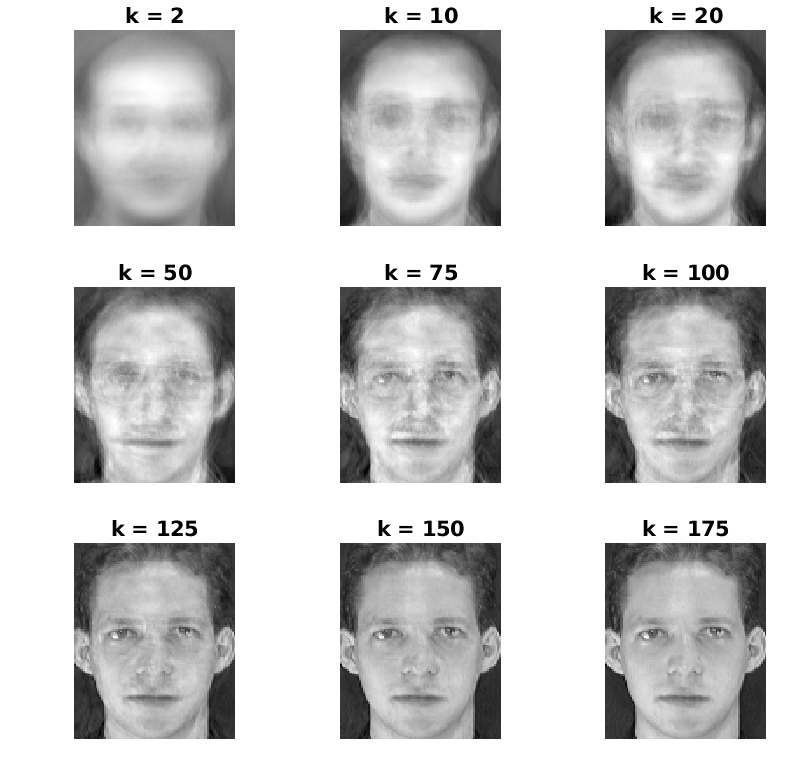
\includegraphics[width=1.34\textwidth]{reconstruct.png}
    	\caption{Reconstruction of images of person 1 \\compressed using various values of k}
	    \label{fig:5.1}
    \end{minipage} \\
\end{figure}

\newpage
\subsection*{5.2: Visualising Eigenfaces}
\quad In this section, we visualise the eigenvectors corresponding to the highest 25 eigenvalues, by reshaping them into a 112x92 dimensional image.
\vspace*{65pt}
\begin{figure}[h!]
    \centering
    \renewcommand{\thefigure}{5.2}
    \begin{minipage}[c][1\width]{0.8\textwidth}
    	\hspace*{-1in}
    	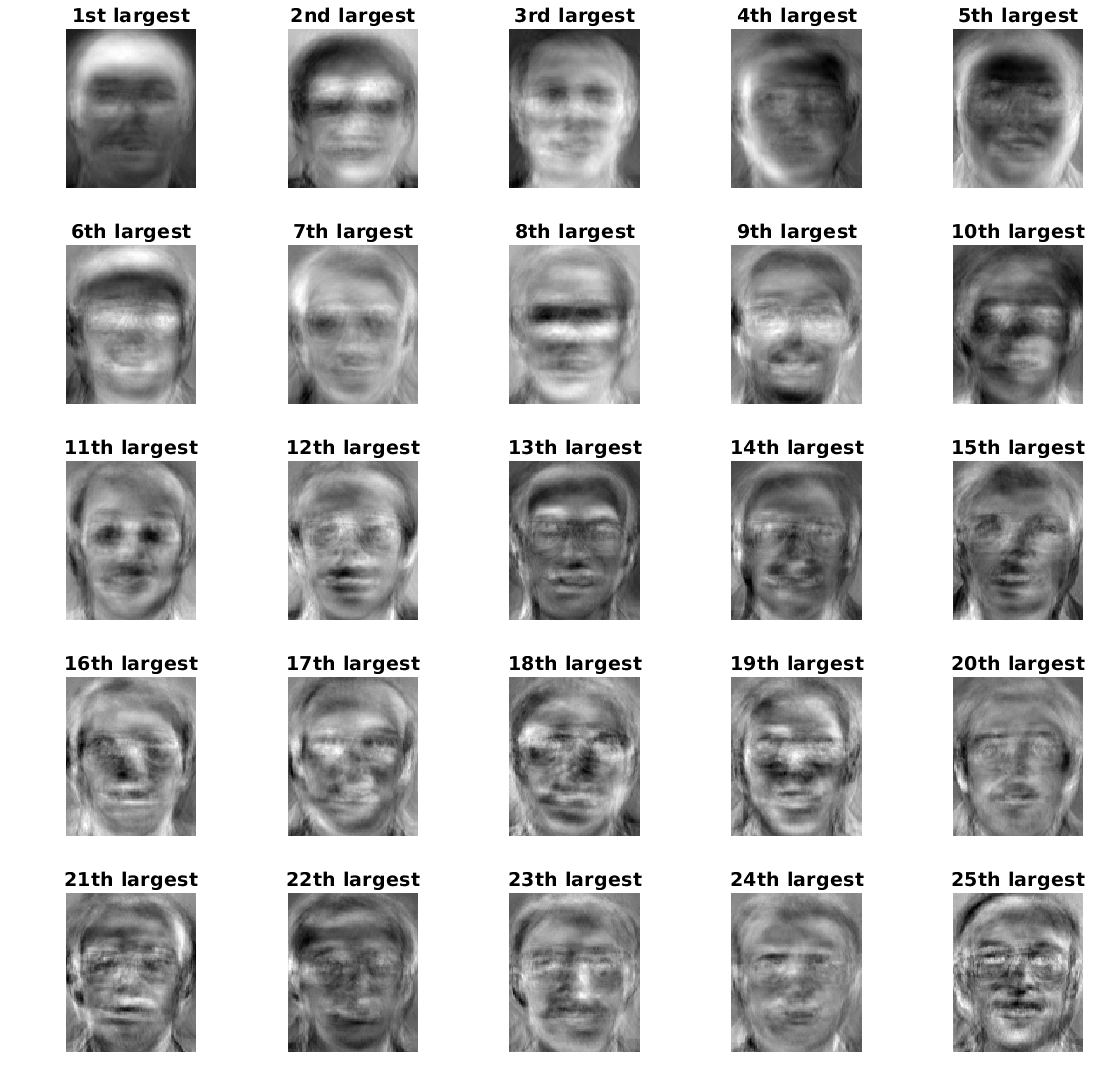
\includegraphics[width=1.34\textwidth]{eigenfaces.png}
    	\caption{Top 25 eigenfaces}
	    \label{fig:5.2}
    \end{minipage} \\
\end{figure}

\newpage
\subsection*{5.3: Usage of code}
\begin{itemize}
\item Execute the \textbf{myMainScript.m} function to display the results and the plots. This takes around 13.5 seconds.

\item Since the dataset is being used for Q4, Q5, Q6 in the assignment, we have kept the datasets in a common directory just inside our submission directory. The ORL dataset is expected to be in a relative directory \textbf{'../../datasets/'}, and the Yale dataset is expected to be in a relative directory \textbf{'../../datasets/CroppedYale/'} \\ 
That is the per person directories should be as follows: \\\textbf{'../../datasets/ORL/s*/'} and \\\textbf{'../../datasets/CroppedYale/yaleB**/'}

\item The \textbf{loadOrl.m} function loads the data.

\item The \textbf{fitPCA.m} function generates the eigenvectors of the data matrix using the $svd$ library function.

\item The \textbf{getPredictor.m} functions returns a struct which stores the relevant eigenvectors, and the subspace transformation operator using the said eigenvectors.

\end{itemize}
\end{document}
